\documentclass[10pt]{amsart}
\usepackage{amsfonts}
\usepackage{amsmath}
\usepackage{amsthm}
\usepackage{amscd}

\usepackage[margin=1in]{geometry}
\usepackage[draft]{todonotes}

\usepackage{csquotes}
\usepackage{enumitem}
\usepackage{multicol}
\usepackage{caption}
\usepackage{tikz}
\usepackage{pgfplots}
\usepackage{minted}
\usepackage{nameref}
\usepackage{algpseudocode}
\usepackage{algorithm}
\usepackage{graphics}

\title{2D FEM Report}
\author{Arden Rasmussen}
\date{\today}

\numberwithin{equation}{section}
\definecolor{red}{RGB}{244,67,54}
\definecolor{pink}{RGB}{233,30,99}
\definecolor{purple}{RGB}{156,39,176}
\definecolor{deep-purple}{RGB}{103,58,183}
\definecolor{indigo}{RGB}{117,125,232}
\definecolor{blue}{RGB}{110,198,255}
\definecolor{pale-blue}{RGB}{103,218,255}
\definecolor{cyan}{RGB}{98,239,255}
\definecolor{teal}{RGB}{82,199,184}
\definecolor{green}{RGB}{128,226,126}
\definecolor{pale-green}{RGB}{190,246,122}
\definecolor{lime}{RGB}{255,255,110}
\definecolor{yellow}{RGB}{255,255,114}
\definecolor{amber}{RGB}{255,243,80}
\definecolor{orange}{RGB}{255,201,71}
\definecolor{deep-orange}{RGB}{255,138,80}
\definecolor{brown}{RGB}{169,130,116}

\newenvironment{Figure}
{\par\medskip\noindent\minipage{\linewidth}}
{\endminipage\par\medskip}

\theoremstyle{definition}
\newtheorem{example}{Example}[section]

\newcommand{\pder}[2][]{\frac{\partial#1}{\partial#2}}
\newcommand{\spder}[2][]{\frac{\partial^2 #1}{\partial#2^2}}

\newcommand{\N}{\mathbb{N}}
\newcommand{\R}{\mathbb{R}}

\begin{document}
\maketitle
\begin{multicols}{2}
  \section{Discretization}%
  \label{sec:descretization}

  I have successfully implement a fast construction of an unconstrained
  Delaunay triangulation, but I am currently running into issues with the
  construction of the constrained Delaunay triangulation. I understand the
  method, there is some issue in my first few attempts at the code, so I will
  review the algorithm more and try again to implement it.

  I have implemented the construction of local basis function based upon the
  \emph{barycentric} coordinate system. I need to determine a method to
  implement the construction of the global basis functions. The global basis
  functions should be a piecewise combination of $N$ different local basis
  functions which all have their peak at a given vertex. The difficulty is that
  each of the parts of the piecewise is dependent on which triangular element
  the point of evaluation is within. Thus I need to develop an efficient method
  for determining the triangle in the mesh that a point is contained within.
  With such a method, the evaluation of the global basis functions will be
  trivial.

  \section{Numerical Approximation}%
  \label{sec:numerical_approximation}
  
  I have a fully functional and surprisingly accurate numerical integration
  over a triangle, which uses the barycentric coordinates and a set of points
  and weights to evaluate the integral on the triangular domain. Its an
  extension of Gaussian quadrature integration, just expanded into 2d and for a
  triangle. Currently I have mine enabled to be accurate up to a degree $8$
  polynomial, which I believe to be sufficient for most cases that the FEM will
  need it for.

  I have also looked further into the residual approximation of sparse
  matrices, and the krylov spaces. I haven't much opportunity to create an
  implementation of it yet, but I will likely do so this weekend.

  \section{Post processing}%
  \label{sec:postprocessing}

  A very important thing to to be able to display the images of the generated
  results. So I have put some work into implementing a method for generating
  the two dimensional images of the domains. So far I have implemented a system
  to accept an arbitrary function from $\R^2\rightarrow \R$ and it utilizes
  color maps to display the $z$ value of the function. I have also implemented
  the use of mesh based domains, where only points within the mesh are
  evaluated and plotted. Again with the same issue as above, I can only get
  this to work nicely with strictly convex meshes.

  I still need to implement text rendering so that I can add $X$, $Y$, and $Z$
  axis labels, and I want to add a legend as well, which should not be too
  difficult.

  \begin{Figure}
     \begin{center}
      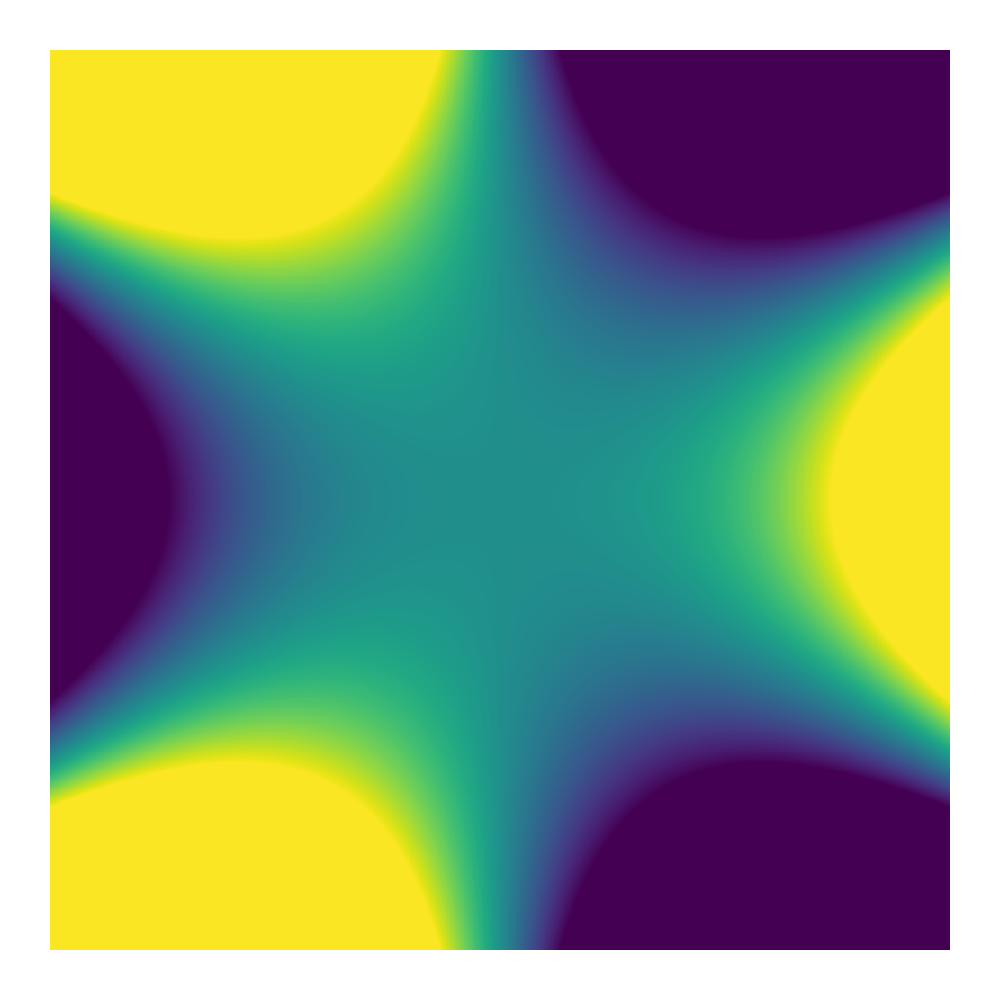
\includegraphics[width=0.6\linewidth]{testing.png}
     \end{center}
     \captionof{figure}{$z=x^3-3xy^2$ on $(-5,-5)$ to $(5,5)$}
  \end{Figure}

  \begin{Figure}
     \begin{center}
      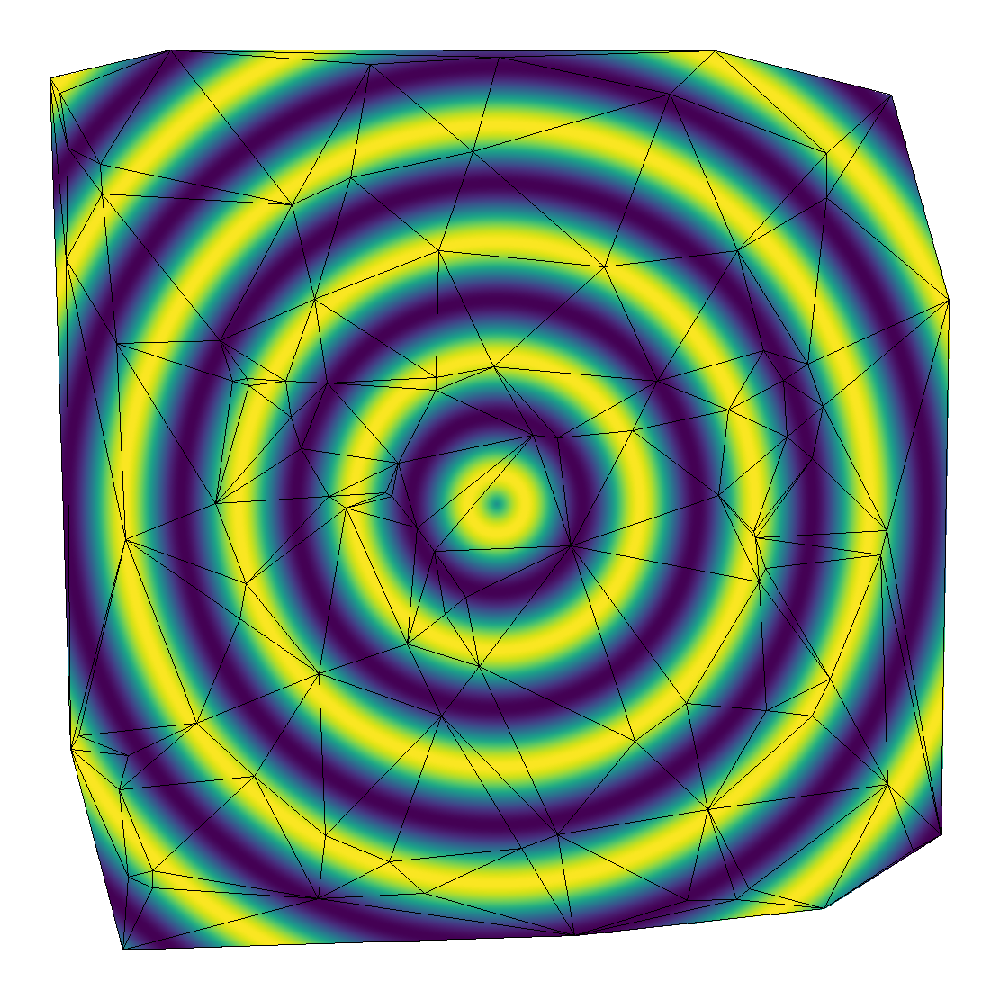
\includegraphics[width=0.7\linewidth]{mesh.png}
     \end{center}
     \captionof{figure}{$z=\sin(0.05*\sqrt{x^2+y^2})$ on a mesh}
  \end{Figure}

\end{multicols}
\end{document}
